% 原书 p.126–p.133（PDF p.134–p.141）
% 第 5 章 5.4 节：无穷维 Morse 理论（$\infty$-dimensional Morse Theory）
% 注意：本文件不写 \chapter（章标题由 ch05a 负责）；5.5 节从 p.141 中部开始，见 ch05b-s03.tex。

\section{无穷维 Morse 理论（\texorpdfstring{$\infty$}{infinity}-dimensional Morse Theory）}
% >>> p134

\begin{keytakeaways}
\begin{itemize}
  \item 几何图像：把「闭轨」看成自由环路空间 $\Lambda_0M$ 上的临界点，于是 Morse 理论的刚性
        可以搬到哈密顿动力学上——这就是无穷维 Morse 理论（Hamilton Floer 同调）的出发点。
  \item 数学工具：辛作用量泛函 $\mathcal{A}_H$、其梯度流方程（一条「扰动」的 $J$-全纯曲线方程）、
        模空间 $\mathcal{M}_{\mathcal{A}_H,\langle\cdot,\cdot\rangle}(x,y)$，以及 Floer 边界算子。
  \item 本节结论：在辛非球面条件 (5.16) 下，$\mathrm{CF}_*(M,\omega;H,J)$ 是链复形，其同调
        $\mathrm{HF}_*(M,\omega;H,J)$ 与 $(H,J)$ 的选取无关，且同构于 $H_*(M;\mathbf{k})$（定理 5.4.1）；
        由此立即得到辛非球面情形的 Arnold 猜想 5.3.1。
  \item 阅读要点：本节与有限维 Morse 理论有三处实质差别——新指标（5.5 节）、无穷维模空间的
        流形结构/横截性、以及冒泡（bubbling）；辛非球面条件正是为排除冒泡而设。
\end{itemize}
\end{keytakeaways}

给定辛流形 $(M,\omega)$。若它满足通常写成如下形式的条件，则称它是\textbf{辛非球面的}
（symplectically aspherical）：
\begin{equation}\tag{5.16}
  \omega(\pi_2(M))=0\qquad\text{且}\qquad c_1(\pi_2(M))=0.
\end{equation}
第一个条件等价于
\[
  \int_{S^2}f^*\omega=0
\]
对任何光滑映射 $f\colon S^2\to M$ 成立；第二个条件则更精细。这里 $c_1=c_1(TM)\in H^2(M;\Z)$
表示 $TM$ 的第一 Chern 类，它是良定义的，因为辛流形的约化结构群是 $\mathrm{Sp}(2n)$，而由
练习 1.5.1 之后紧接的性质 (iii)，$\mathrm{Sp}(2n)$ 等价于 $\mathrm{U}(n)$，这与复结构的
情形完全相同。关于这一点的更多细节见 5.5 节。第二个条件更严格的写法是
$c_1(TM)|_{\operatorname{im}\bigl(h_2\colon\pi_2(M)\to H_2(M;\Z)\bigr)}=0$，其中 $h_2$ 是
第二 Hurewicz 映射。
% [Tutor Note: 易错预警（记号约定）——(1) $c_1(\pi_2(M))=0$ 是简写，准确含义是
%  $\langle c_1(TM),u_*[S^2]\rangle=0$ 对一切 $u\colon S^2\to M$ 成立，即 $c_1$ 在 Hurewicz 像
%  $\operatorname{im}h_2$ 上取零（$h_2$ 未必满，故不能说 $c_1=0$）。(2) $\mathrm{Sp}(2n)$ 与
%  $\mathrm{U}(n)$ 的等价只是「极大紧子群」意义下的同伦等价，用来说明 $TM$ 作为复向量丛的
% 第一 Chern 类有定义，并不意味着辛结构自带复结构。(3) 这两个条件正是为了在定义 Floer 边界
%  算子时避免球面带来的「冒泡」与「多重覆盖」项，见本节末尾的注 5.4.5。]

\begin{wexam}{5.4.1}
  对例 1.2.3 中讨论的任何闭定向曲面 $(\Sigma_g,\omega_{\mathrm{area}})$，当 $g\geqslant1$ 时它是
  辛非球面的，因为 $\pi_2(\Sigma_{g\geqslant1})=0$。\hfill$//$
\end{wexam}

\begin{wrem}{5.4.1}
  在第 8 章开头我们将看到，为简化 Floer 理论或类似理论的构造框架，人们会对辛流形附加包括 (5.16)
  在内的各种条件。
\end{wrem}

记 $\Lambda M$ 为 $(M,\omega)$ 的\textbf{自由环路空间}（free loop space）。在其中，$\Lambda_0M$
表示 $\Lambda M$ 里由所有可缩环路组成的连通分支。给定哈密顿函数 $H\colon[0,1]\times M\to\R$，
我们的目标是在 $\Lambda M$ 或 $\Lambda_0M$ 上构造一个「Morse 函数」，使它的临界点捕获某些
哈密顿动力学信息。于是 Morse 理论提供的刚性将蕴涵哈密顿动力学的刚性。

为此，考虑 $x=x(t)\in\Lambda_0M$。由于它可缩，我们可以选取一个\textbf{界定圆盘}
（bounding disk）$w\colon\mathbb{D}^2\to M$，使得 $w(\partial\mathbb{D}^2)=x$。再考虑一个称为
\textbf{辛作用量泛函}（symplectic action functional）的泛函，其定义为
\begin{equation}\tag{5.17}
  \mathcal{A}_H\bigl((x,w)\bigr):=-\int_{\mathbb{D}^2}w^*\omega
    +\int_0^1H\bigl(t,x(t)\bigr)\dd t.
\end{equation}
上面 (5.16) 中的第一个条件保证 $\mathcal{A}_H((x,w))$ 与界定圆盘的选取无关。事实上，若
$w'\colon\mathbb{D}^2\to M$ 是环路 $x$ 的另一个界定圆盘，则 $\overline{w}\#w'$ 表示 $\pi_2(M)$
中的一个类（见图 5.16），其中 $\overline{w}$ 表示把 $w$ 取反向定向。
% [Tutor Note: 易错预警——(1) $\overline{w}\#w'$ 的构造：沿公共边界 $\partial\mathbb{D}^2=x$
%  把 $w$ 的定向反转后与 $w'$ 粘合，得到 $S^2\to M$ 的一个映射，故给出 $\pi_2(M)$ 的类；
%  矩阵记号上也可读作 $[w']-[w]\in\pi_2(M)$（在 $\pi_2$ 为阿贝尔群时）。(2) 请核对
%  (5.17) 中两项的符号：作用量泛函的符号约定（$-\int\omega$ 还是 $+\int\omega$、$\int H\dd t$
%  的符号）直接决定 (5.17)--(5.18) 及后面梯度流方程的写法；本书取 $-\int_{\mathbb{D}^2}w^*\omega
%  +\int_0^1H\dd t$，与 $-\dd F=\omega(X_F,\cdot)$ 的约定配套。]

由于 $\omega$ 在 $\pi_2(M)$ 上为零，我们有 $\mathcal{A}_H((x,w))=\mathcal{A}_H((x,w'))$。因此，
在辛非球面条件 (5.16) 下，(5.17) 所定义的辛作用量泛函是 $\Lambda_0M$ 上良定义的泛函。

% >>> p135
\begin{figure}[htbp]
  \centering
  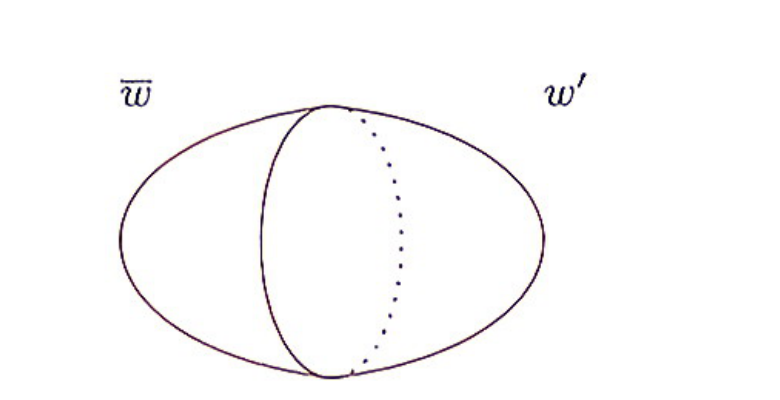
\includegraphics[width=0.42\linewidth]{figures/fig_p135_1.png}
  \caption*{图 5.16\quad 粘合 $\overline{w}$ 与 $w'$（原书 p.127, Figure 5.16）}
\end{figure}

\begin{wprop}{5.4.1}
  设 $(M,\omega)$ 是辛非球面的辛流形，$H\colon[0,1]\times M\to\R$ 是哈密顿函数。则由 (5.17)
  定义的作用量泛函 $\mathcal{A}_H\colon\Lambda_0M\to\R$ 具有下述性质：
  \begin{equation*}
  \begin{aligned}
    \Crit(\mathcal{A}_H)
      &=\bigl\{\{\varphi_H^t\}_{t\in[0,1]}\text{ 的可缩闭哈密顿轨道}\bigr\}\\
      &=\bigl\{x\in\Lambda_0M\ \big|\ \dot x(t)=X_H(x(t))\bigr\},
  \end{aligned}
  \end{equation*}
  其中 $X_H$ 表示 $H$ 的哈密顿向量场。
\end{wprop}
% [Tutor Note: 易错预警——第二条等式把 $\mathcal{A}_H$ 看成 $\Lambda_0M$ 上的泛函，这在 (5.17)
%  中依赖界定圆盘 $w$；之所以能这样写，正是因为辛非球面条件保证 $\mathcal{A}_H$ 不依赖 $w$
%  的选取（见上一段）。另请注意「闭轨道」与「周期轨道」的区别：$\dot x=X_H(x)$ 的解自动满足
%  $x(1)=\varphi_H^1(x(0))$，故它是时间-1 意义下的闭轨道；而 $\Crit(\mathcal{A}_H)$ 中的元素
%  要求 $x(0)=x(1)$，即它同时是 $\varphi_H^1$ 的不动点。]

\begin{wrem}{5.4.2}
  观察到 $\Crit(\mathcal{A}_H)$ 可以等同于哈密顿流 $\{\varphi_H^t\}_{t\in[0,1]}$ 的时间-1 映射
  $\varphi_H^1$ 的不动点集的一个子集。
\end{wrem}

\begin{wproof}[命题 5.4.1 的证明]
  回忆对任意 $x\in\Lambda M$，沿 $x$ 的切向量是
  $T_x\Lambda M=\{\xi=\xi(t)\mid\xi(t)\in T_{x(t)}M\}$，它等于 $x^*TM$ 在环路 $x$ 上的截面
  的集合。为计算 $\dd\mathcal{A}_H((x,w))(\xi)$，即 $\mathcal{A}_H$ 在点 $(x,w)$ 处沿方向
  $\xi\in T_x\Lambda M$ 的导数，我们把 $x(t)$ 延拓为 $\tilde x(s,t)$，$s\in(-\epsilon,\epsilon)$，
  使得
  \[
    \tilde x(0,t)=x(t)\qquad\text{且}\qquad
    \frac{\partial\tilde x}{\partial s}(0,t)=\xi(t).
  \]
  示意图见图 5.17。

  \begin{figure}[htbp]
    \centering
    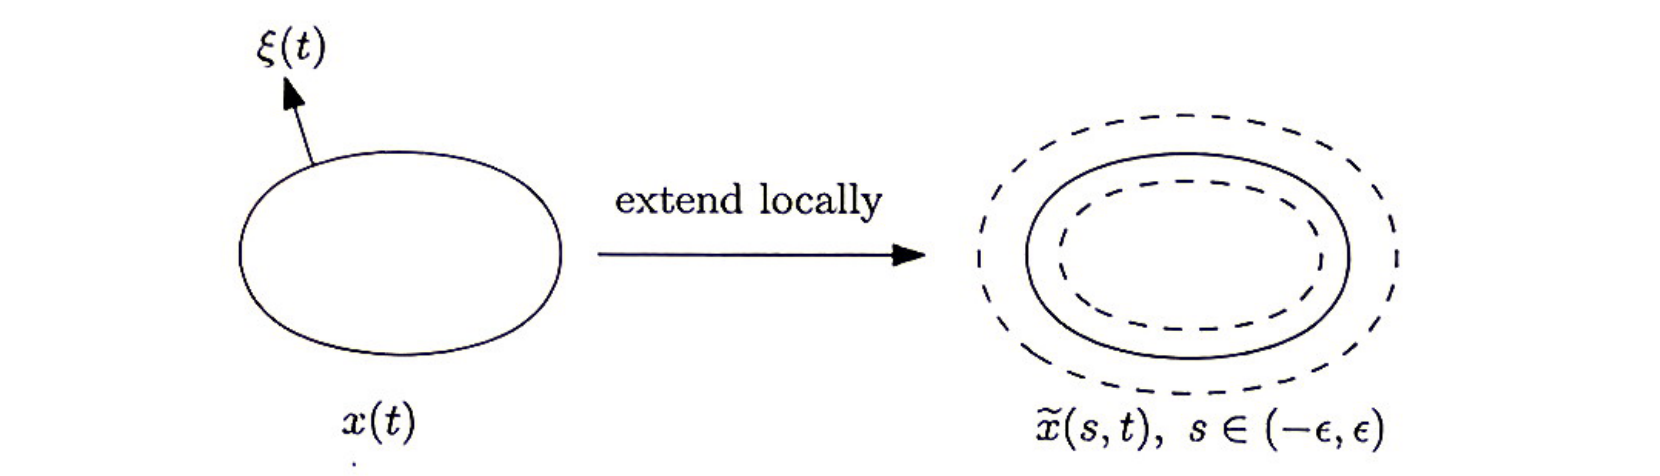
\includegraphics[width=0.72\linewidth]{figures/fig_p135_2.png}
    \caption*{图 5.17\quad $x(t)$ 的延拓（原书 p.127, Figure 5.17）}
  \end{figure}

  类似地，对每个 $s\in(-\epsilon,\epsilon)$，取界定圆盘 $\tilde w(s,\cdot)$ 作为 $w$ 的局部
  延拓。示意图见图 5.18。

  向量场 $\xi$ 先延拓为定义在 $w$ 上的 $\xi'$，再进一步延拓为定义在 $\tilde w$ 上的向量场。于是
  \begin{equation*}
    \mathcal{A}_H\bigl((\tilde x(s,\cdot),\tilde w(s,\cdot))\bigr)
      =-\int_{\mathbb{D}^2}\bigl(\tilde w(s,\cdot)\bigr)^*\omega
        +\int_0^1H\bigl(t,\tilde x(s,t)\bigr)\dd t.
  \end{equation*}

% >>> p136
  \begin{figure}[htbp]
    \centering
    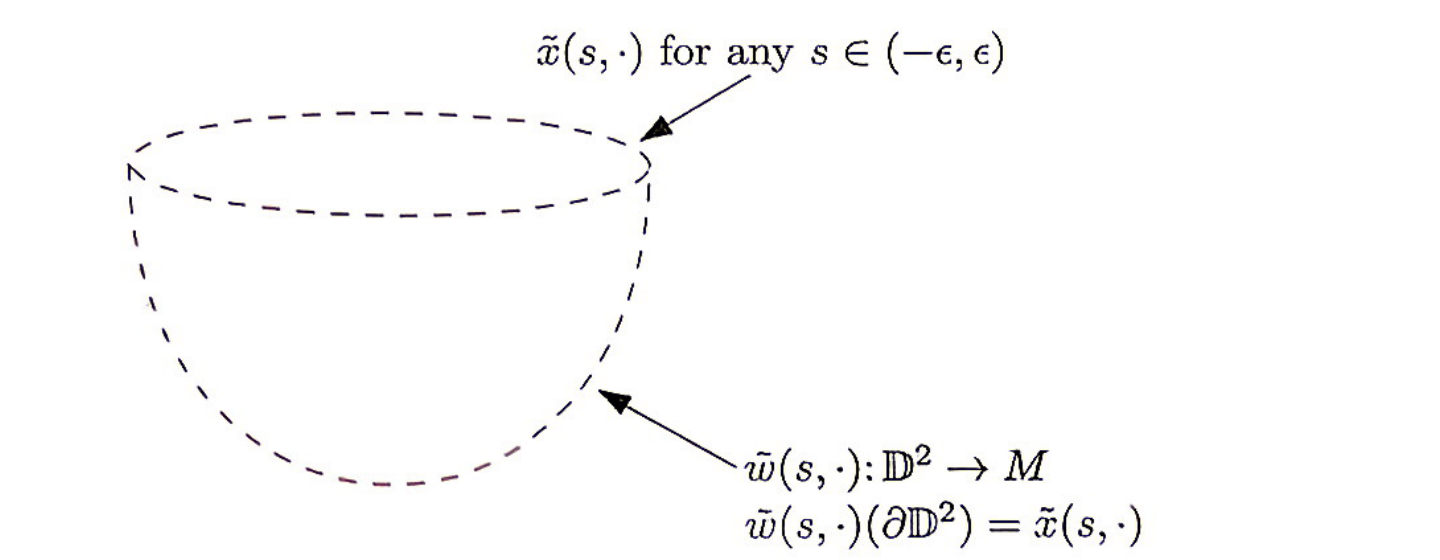
\includegraphics[width=0.58\linewidth]{figures/fig_p136_1.png}
    \caption*{图 5.18\quad $w$ 的局部延拓（原书 p.128, Figure 5.18）}
  \end{figure}

  将上式对 $s$ 求导（并在 $s=0$ 处取值），得到
  \[
    \frac{\dd}{\dd s}\mathcal{A}_H\bigl((\tilde x(s,\cdot),\tilde w(s,\cdot))\bigr)
      \Big|_{s=0}
      =-\int_{\mathbb{D}^2}\frac{\dd}{\dd s}\bigl(\tilde w(s,\cdot)\bigr)^*\omega
        \Big|_{s=0}
       +\int_0^1\frac{\dd}{\dd s}H\bigl(t,\tilde x(s,t)\bigr)\Big|_{s=0}\dd t.
  \]
  第一项等于
  \[
  \begin{aligned}
    \int_{\mathbb{D}^2}\frac{\dd}{\dd s}\bigl(\tilde w(s,\cdot)\bigr)^*\omega\Big|_{s=0}
      &=\int_{\mathbb{D}^2}w^*\bigl(\mathcal{L}_{\xi'}\omega\bigr)
       =\int_{\mathbb{D}^2}w^*\bigl(\dd\iota_{\xi'}\omega\bigr)\\
      &=\int_{\mathbb{D}^2}\dd w^*\bigl(\iota_{\xi'}\omega\bigr)
       =\int_{S^1}x^*\bigl(\iota_{\xi}\omega\bigr)
       =\int_0^1\omega\bigl(\xi(t),\dot x(t)\bigr)\dd t.
  \end{aligned}
  \]
  % [Tutor Note: 易错预警（符号约定）——严格地，上面这个「第一项」在求导式中带负号，即
  %  $\dd\mathcal{A}_H$ 的第一部分为 $-\int_{\mathbb{D}^2}\frac{\dd}{\dd s}(\cdots)^*\omega|_{s=0}$；
  %  原文在「第一项等于」这一行把外层负号省略了，而链式等式的其余部分与结论 (5.18) 均正确。
  %  请按「带负号的第一项 $=-\int_0^1\omega(\xi,\dot x)\dd t$」阅读，再与下面的第二项相减相加。
  %  详见 qsg/notes/review_ch05b.md。]
  第二项等于
  \[
  \begin{aligned}
    \int_0^1\frac{\dd}{\dd s}H\bigl(t,\tilde x(s,t)\bigr)\Big|_{s=0}\dd t
      &=\int_0^1\dd H\bigl(t,x(t)\bigr)\bigl(\xi(t)\bigr)\dd t\\
      &=-\int_0^1\omega\bigl(X_H(x(t)),\xi(t)\bigr)\dd t
       =\int_0^1\omega\bigl(\xi(t),X_H(x(t))\bigr)\dd t.
  \end{aligned}
  \]
  因此，$\dd\mathcal{A}_H((x,w))(\xi)=0$ 等价于
  \begin{equation}\tag{5.18}
    \int_0^1\omega\bigl(\xi(t),X_H(x(t))-\dot x(t)\bigr)\dd t=0.
  \end{equation}
  由于这对任意 $\xi$ 都成立，等式 (5.18) 等价于 $\dot x(t)=X_H(x(t))$。这就完成了证明。
\end{wproof}

% [Tutor Note: 含糊点拨——第三行到第四行用了 Stokes 公式（准确说是「区域上的恰当形式之积分
%  $=$ 边界上的积分」），并注意 $\partial\mathbb{D}^2=S^1$ 的定向：$\int_{\mathbb{D}^2}\dd\eta
% =\int_{\partial\mathbb{D}^2}\eta$ 的定向约定决定了 $\int_{S^1}x^*(\iota_\xi\omega)$ 的符号。
% 若把 $S^1$ 的定向或 $w$ 的定向改成相反，此处会出现一个负号，请以 (5.18) 的最终形式为锚点
% 逐符号复核。另：$\dd H(\xi)=-\omega(X_H,\xi)$ 一步用了本书约定 $\iota_{X_H}\omega=-\dd H$。]

命题 5.4.1 在切触几何中有类似的版本。

\begin{wexer}{5.4.1}
  设 $(M,\xi=\ker\alpha)$ 是带固定切触 1-形式 $\alpha$ 的切触流形。考虑如下定义的作用量泛函
  $\mathcal{A}_\alpha\colon\Lambda M\to\R$：
  \[
    \gamma\mapsto\mathcal{A}_\alpha(\gamma):=\int_\gamma\alpha.
  \]
% >>> p137
  证明：$\gamma\in\Crit(\mathcal{A}_\alpha)$ 当且仅当 $\gamma$ 是一条周期为
  $\mathcal{A}_\alpha(\gamma)$ 的闭 Reeb 轨道。
\end{wexer}

为确认泛函 $\mathcal{A}_H$ 确实是 $\Lambda_0M$ 上的 Morse 函数（泛函），我们需要验证：在每个
$x\in\Crit(\mathcal{A}_H)$ 处，$\mathcal{A}_H$ 在 $x$ 的 Hessian 是非退化的。这需要仔细计算，
而且事实上它只在 $x$ 满足某种「非退化」条件时才成立。

\begin{wdefn}{5.4.1}
  哈密顿同痕 $\{\varphi_H^t\}_{t\in[0,1]}$ 的闭哈密顿轨道 $x=x(t)$ 称为\textbf{非退化的}
  （non-degenerate），如果
  \[
    \det\Bigl(\mathbf{1}-(\varphi_H^1)_{*}\big|_{x(0)}\Bigr)\ne0,
  \]
  其中 $(\varphi_H^t)_{*}\colon T_{x(0)}M\to T_{x(t)}M$ 是沿轨道 $x(t)$ 的前推（特别地，
  $(\varphi_H^1)_{*}$ 把 $T_{x(0)}M$ 映到自身）。若哈密顿函数 $H$ 的所有闭哈密顿轨道都非退化，
  则称 $H$ 是\textbf{非退化的}。
\end{wdefn}
% [Tutor Note: 易错预警——(1) 这里 $\mathbf{1}$ 表示 $T_{x(0)}M$ 上的恒等算子（$2n\times2n$
%  矩阵），行列为 $\det(\mathbf{1}-d\varphi_H^1(x(0)))$；下标 $*$ 的取法（前推还是拉回）与
%  矩阵的基选取有关，但行列式是否为零与之无关。(2) 「非退化」是开条件（对 $(H,J)$ 通有成立），
%  其含义是 $1$ 不是线性化返回映射的特征值，等价于 $\mathrm{graph}(\varphi_H^1)$ 与对角线横截
%  （注 5.4.3）。(3) 请注意它与「$\mathcal{A}_H$ 的 Hessian 非退化」的等价性不是自动的，而正是
%  下一段要验证的内容；在无穷维情形 Hessian 是 Fredholm 算子，其非退化性须另行讨论。]

\begin{wrem}{5.4.3}
  可以验证：$H$ 非退化，当且仅当 $\mathrm{graph}(\varphi_H^1)$ 在乘积 $M\times M$ 中与对角线
  $\Delta$ 横截。
\end{wrem}

\begin{wexer}{5.4.2}
  考虑 Morse 函数 $F\colon(M,\omega)\to\R$。我们可以把它视为与时间无关的哈密顿函数。临界点
  $p\in\Crit(F)$ 当然是一条闭哈密顿轨道（常值轨道）。证明：若 $p$ 作为闭哈密顿轨道是非退化的
  （按定义 5.4.1），则它是 $F$ 的非退化临界点。因此，对与时间无关的 Morse 函数 $F$，若它在
  哈密顿意义下非退化，则它在 Morse 意义下也非退化。

  上述命题的逆命题成立吗？若成立，请证明；否则请给出反例（参看练习 5.5.1）。
\end{wexer}
% [Tutor Note: 含糊点拨——练习 5.4.2 的逆命题是关键：取 $F$ 为 Morse 函数，$p$ 是 $F$ 的非退化
%  临界点（Hessian 非奇异），但作为时间-1 映射的不动点，其线性化返回映射是
%  $d\varphi_F^1(p)=\exp\bigl(\mathbf{1}\cdot\nabla^2F\text{ 的某个}\ J\text{-线性化}\bigr)$，
%  只有当 $\varphi_F^1$ 的线性化没有特征值 $1$ 时才非退化。一般情形二者并不等价（这解释了原文
%  为何把它留作练习，并指向练习 5.5.1）。]

与有限维 Morse 情形类似，我们将研究连接 $\mathcal{A}_H$ 的两个（不同）临界点的负梯度流线。
为此，我们需要 $\Lambda M$ 上的一个度量，特别是在子流形 $\Lambda_0M$ 上。

固定 $M$ 上一个 $\omega$-相容的近复结构 $J$（它按 (1.8) 的方式在 $M$ 上诱导度量 $g_J$）。它
在 $\Lambda_0M$ 上诱导一个度量，具体写为
\begin{equation}\tag{5.19}
  \langle\xi,\eta\rangle(x):=\int_0^1g_J(x(t))\bigl(\xi(t),\eta(t)\bigr)\dd t
    \ \Bigl(=\int_0^1\omega_{x(t)}\bigl(\xi(t),J\eta(t)\bigr)\dd t\Bigr),
\end{equation}
其中 $x\in\Lambda_0M$，$\xi,\eta\in T_x\Lambda_0M$。按定义，梯度向量场
$\nabla_{\langle\cdot,\cdot\rangle}\mathcal{A}_H$（简记为 $\nabla\mathcal{A}_H$）是由下述等式
定义的 $\Lambda M$ 上的向量场：
\[
  \bigl\langle\nabla\mathcal{A}_H(x(t)),\xi\bigr\rangle
    =\dd\mathcal{A}_H(x(t))\bigl(\xi(t)\bigr)
    =\int_0^1\omega_{x(t)}\bigl(\xi(t),X_H(x(t))-\dot x(t)\bigr)\dd t,
\]
而由 (5.19)，我们还有
\[
  \bigl\langle\nabla\mathcal{A}_H(x(t)),\xi\bigr\rangle
    =\int_0^1\omega_{x(t)}\bigl(\nabla\mathcal{A}_H(x(t)),J\xi(t)\bigr)\dd t.
\]

% >>> p138
因此，梯度向量场由下式给出：
\begin{equation}\tag{5.20}
  \nabla\mathcal{A}_H(x(t))=-J(x(t))\bigl(X_H(x(t))-\dot x(t)\bigr).
\end{equation}
% [Tutor Note: 易错预警——由 (5.19) 的第二个等式反解 (5.20) 时，请核对 $J$ 作用在哪一侧：
%  约定 $g_J(u,v)=\omega(u,Jv)$ 下，$\omega(\xi,X_H-\dot x)=g_J(\xi,J(X_H-\dot x))$，
%  于是 $\nabla\mathcal{A}_H=J(X_H-\dot x)$ 还是 $-J(X_H-\dot x)$ 取决于 $g_J(u,v)$ 中 $J$ 的
%  位置以及 $\omega$ 的次序。本书的最终答案是 (5.20)（带负号），它与 (5.21) 及梯度流方程
%  $\partial_su=-\nabla\mathcal{A}_H$ 相互印证；换约定时请整条链一致改号。]

与 Morse 情形 (5.2) 一样，$\mathcal{A}_H$ 的负梯度流线（连接 $x,y\in\Crit(\mathcal{A}_H)$）
作为 $\Lambda_0M$ 中的 $1$ 维曲线，在几何上由柱面 $u(s,t)\colon\R\times S^1\to M$ 实现
（见图 5.19）。

\begin{figure}[htbp]
  \centering
  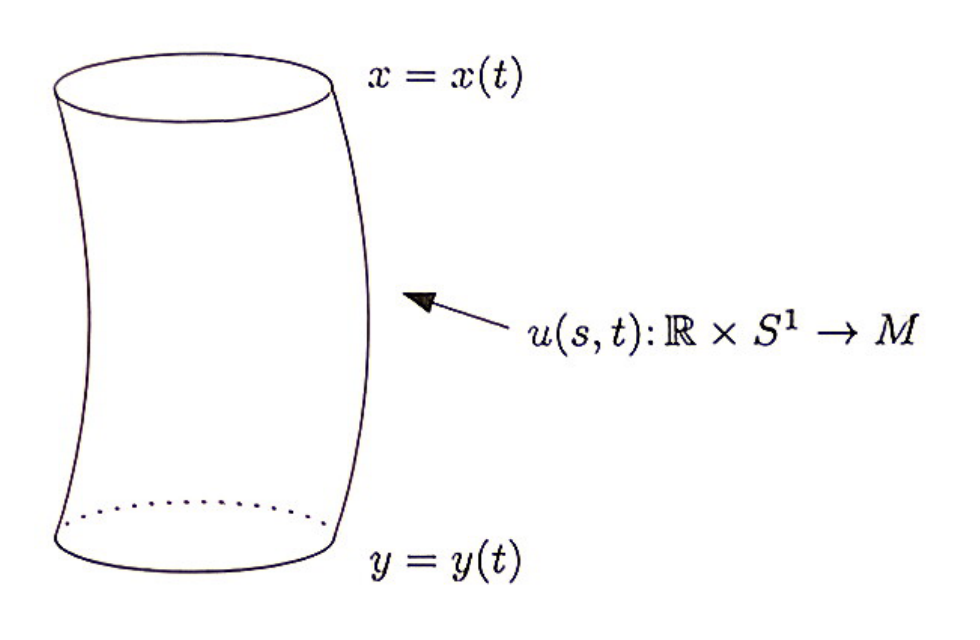
\includegraphics[width=0.42\linewidth]{figures/fig_p138_1.png}
  \caption*{图 5.19\quad 负梯度流线 $u(s,t)$ 连接 $x$ 与 $y$（原书 p.130, Figure 5.19）}
\end{figure}

更具体地，由 (5.20)，$u(s,t)$ 满足下述方程
\[
  \frac{\partial u}{\partial s}(s,t)=-\nabla\mathcal{A}_H(u(s,t))
    =J(u(s,t))\Bigl(X_H(u(s,t))-\frac{\partial u}{\partial t}(s,t)\Bigr).
\]
整理各项，它等价于
\begin{equation}\tag{5.21}
  \Bigl(\frac{\partial u}{\partial s}(s,t)
    +J(u(s,t))\frac{\partial u}{\partial t}(s,t)\Bigr)
    -J(u(s,t))X_H(u(s,t))=0.
\end{equation}

\begin{wrem}{5.4.4}
  有时 (5.21) 中的项 $J(u)X_H(u)$ 也写作 $\nabla_{g_J}H(u)$。确实，由两个关系式
  $\omega(\cdot,X_H)=\dd H(\cdot)=g_J\bigl(\nabla_{g_J}H,\cdot\bigr)$ 与
  $\omega(\cdot,J\nabla_{g_J}H)=\omega(\cdot,X_H)$，可知
  $\nabla_{g_J}H=-JX_H$。
\end{wrem}

回忆称 $u\colon(\Sigma,j)\to(M,\omega,J)$ 是一条 $J$-全纯曲线，如果 $J\circ\dd u=\dd u\circ j$。
在 Riemann 曲面 $(\Sigma,j)$ 的局部坐标 $(s,t)$ 中（允许有穿孔），它等价于 Cauchy--Riemann 型
方程 $\frac{\partial u}{\partial s}(s,t)+J(u(s,t))\frac{\partial u}{\partial t}(s,t)=0$
（见 (3.17)）。于是 (5.21) 可以看作一条「扰动」的 $J$-全纯曲线。人们会期望 $J$-全纯曲线的
分析性质能够推广到满足 (5.21) 的曲线。事实上，对许多基本结果这确实成立（例如见 [229] 的
第 6.2 节）。

接下来，对给定的辛流形 $(M,\omega)$、$\omega$-相容的近复结构 $J$ 以及
$x,y\in\Crit(\mathcal{A}_H)$，我们考虑下述模空间，它是模空间 (5.3) 的类比：
\[
  \mathcal{M}_{\mathcal{A}_H,\langle\cdot,\cdot\rangle}(x,y)
  =\left\{\,u(s,t)\colon\R\times S^1\to M
    \ \middle|\
    \begin{array}{l}
      u(s,t)\text{ 满足 (5.21)}\\[1pt]
      \displaystyle\lim_{s\to\infty}u(s,t)=x(t)\\[2pt]
      \displaystyle\lim_{s\to-\infty}u(s,t)=y(t)
    \end{array}
    \right\}\Big/\R\text{-平移}.
\]

% >>> p139
它由所有从 $x$ 出发、到达 $y$ 的 $\mathcal{A}_H$ 的负梯度流线组成，模去 $\R$-平移
$r\cdot u(s,t):=u(s+r,t)$。
% [Tutor Note: 含糊点拨——模空间的记号 $\mathcal{M}_{\mathcal{A}_H,\langle\cdot,\cdot\rangle}(x,y)$
%  中，下标 $\langle\cdot,\cdot\rangle$ 记录所用的度量（由 $J$ 决定的 $L^2$ 度量），这一点在
%  有限维 Morse 情形对应 $\mathcal{M}_F(x,y)$ 依赖于度量 $g$。严格地说，这里的 $\R$-平移
%  只在流线非常值（即 $x\ne y$）时才是自由的；同时须先证明极限 $s\to\pm\infty$ 存在（这依赖
%  于 (5.21) 的先验估计与指数衰减），才能把上式当作集合来写。文献中这些技术细节见
%  Floer 1989 与 Salamon 的综述。]

回忆在 Morse 情形，这类模空间对于构造 Morse 同调群 $\mathrm{HM}_*(F,g;\mathbf{k})$（更确切地说，
Morse 边界算子 $\partial_*$）特别重要。这依赖于下面两个结果：命题 5.1.1 中的指标公式，以及
定理 5.1.1 中的断裂流线。与此相关，本情形将有三处重大差异：

(i)（新指标）由于我们在 $\Lambda_0M$ 这个无穷维空间上工作，由有限维局部表达式 (5.1) 定义的
Morse 指标不再适用。在 5.5 节我们将引入一个在新情形下行之有效的指标。关于这些模空间更系统的
研究，我们推荐一本写得很详细的专著 [19]。

(ii)（流形结构）需要确认：对通有的近复结构 $J$，模空间
$\mathcal{M}_{\mathcal{A}_H,\langle\cdot,\cdot\rangle}(x,y)$ 确实具有流形结构。命题 5.1.1 的证明
基于维数计数，不能直接用于无穷维情形。

(iii)（冒泡问题）由满足 (5.21) 的曲线像 $\{u(s,t)\}_{(s,t)\in\R\times S^1}$ 给出的二维轨迹，
其断裂流线可能含有新的成分——\textbf{冒泡}（bubbling），即可能出现一个完整的 $J$-全纯球面
（见图 5.20）。这一冒泡现象可以在 8.3 节中明确看到。

\begin{figure}[htbp]
  \centering
  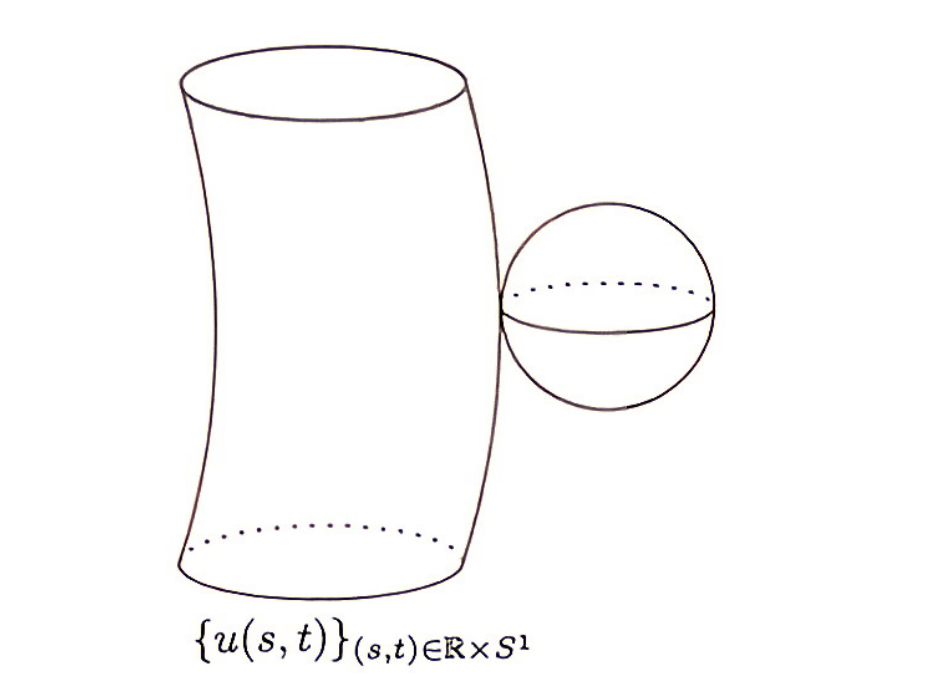
\includegraphics[width=0.42\linewidth]{figures/fig_p139_1.png}
  \caption*{图 5.20\quad $u$ 上的冒泡球面（原书 p.131, Figure 5.20）}
\end{figure}

\begin{wrem}{5.4.5}
  在 $(M,\omega)$ 辛非球面的情形，我们可以忽略上面的第 (iii) 点。否则，设 $A$ 表示冒泡现象中
  $J$-全纯球面所代表的类，则 $\omega(A)=0$（由 (5.16) 的第一个条件）与 $\omega(A)>0$ 矛盾
  （因为 $A$ 的代表是 $J$-全纯的，而命题 1.4.1 蕴涵它必须为正）。
\end{wrem}
% [Tutor Note: 含糊点拨——这里的论证只用到「能量正性」：$J$-全纯球面 $u$ 的 $\omega$-能量
%  $\int u^*\omega=\int|\partial u|^2>0$（在非平凡时），故 $\omega(A)>0$；而辛非球面条件说
%  $\omega$ 在 $\pi_2$ 上为零，矛盾。请注意：$A$ 是 $\pi_2(M)$ 中的类，而 $\omega(A)$ 只依赖
%  于 $A$（由 Stokes 公式），与代表无关。反过来，若去掉辛非球面条件，冒泡项会以「量子修正」
%  的形式进入边界算子，这正是量子上同调/Novikov 环的由来。]

假设我们能够克服上面 (i)、(ii)、(iii) 三点所提出的全部问题，那么按照构造 Morse 同调群的同样
方式，我们便得到一个链复形
% >>> p140
\begin{equation}\tag{5.22}
  \bigoplus_*\mathrm{CF}_*(M,\omega;H,J)
    :=\mathbf{k}\bigl\langle\Crit(\mathcal{A}_H)\bigr\rangle
    =\mathbf{k}\bigl\langle\{\varphi_H^t\}_{t\in[0,1]}\text{ 的可缩周期轨道}\bigr\rangle,
\end{equation}
而 Floer 边界算子则通过在若干模空间 $\mathcal{M}_{\mathcal{A}_H,\langle\cdot,\cdot\rangle}(x,y)$
中计数元素来定义——每当 $x$ 与 $y$ 的指标之差为 $1$ 时，即
\begin{equation}\tag{5.23}
  \partial_*(x)=\sum_{\operatorname{ind}(y)=\operatorname{ind}(x)-1}
    \#_{\Z_2}\mathcal{M}_{\mathcal{A}_H,\langle x,y\rangle}(x,y)\,y.
\end{equation}
于是所得的同调群记作 $\mathrm{HF}_*(M,\omega;H,J)$，称为哈密顿系统 $(M,\omega,H,J)$ 的\textbf{哈密顿
Floer 同调群}。
% [Tutor Note: 易错预警（三处）——(1) $\mathbf{k}\langle S\rangle$ 表示以集合 $S$ 为基的自由
%  $\mathbf{k}$-模；由于 $\Crit(\mathcal{A}_H)$ 可能无穷，这里默认取**直和**（每个次数上有限
%  生成）而非直积，否则边界算子未必良定义。(2) (5.23) 中的 $\#_{\Z_2}$ 表示模 2 计数，说明
%  此处系数域实际上是 $\Z_2$：要换成一般域 $\mathbf{k}$ 或整数系数，必须为每个模空间配上
%  「相干定向」（coherent orientation），这是 Floer 理论中一项独立的技术工作；原文 (5.22)
%  写 $\mathbf{k}$、(5.23) 写 $\#_{\Z_2}$，两处系数并不完全统一，属常见的记号省略。
%  (3) $\operatorname{ind}$ 在无穷维情形必须换成 5.5 节的 Conley--Zehnder 指标；它取代有限维
%  Morse 指标，但一般只是整数（不必与 Morse 指标同号），见例 5.5.7 的 μ_CZ = 3 与
%  Morse 指标 0 之对比。]

下述结果是定理 5.1.2 的类比（但证明更高级，条件也更严格）。

\begin{wthm}{5.4.1}（[83,195]）
  设 $(M,\omega)$ 是辛非球面的辛流形，$(H,J)$ 由非退化哈密顿函数
  $H\colon M\times[0,1]\to\R$（见定义 5.4.1）与通有的 $\omega$-相容近复结构 $J$ 组成。则对任意
  两个这样的配对 $(H,J)$ 与 $(H',J')$，有
  \[
    \mathrm{HF}_*(M,\omega,H,J)\cong\mathrm{HF}_*(M,\omega,H',J').
  \]
  此外，$\mathrm{HF}_*(M,\omega,H,J)\cong H_*(M;\mathbf{k})$，即 $X$ 的经典同调群（系数域为
  $\mathbf{k}$）。
\end{wthm}
% [Tutor Note: 原文疑误——定理陈述末句的「$X$ 的经典同调群」中 $X$ 无定义，应为 $M$。译文保留
%  原文写法 $X$，但请按 $M$ 理解；详见 qsg/notes/review_ch05b.md。另请注意本定理有两部分：
%  第一部分是 $(H,J)$ 的独立性（延拓映射/同伦论证），第二部分是同调群与经典同调的同构
%  （可用 Morse 情形 $H$ 极小、$J$ 与 $H$ 的梯度相容的特殊选取来验证）。]

这一定理可以从一个更强的结果——定理 6.2.1（见注 6.2.3）——导出，只需假定
$\mathrm{HF}_*(M,\omega,H,J)$ 的良定义性。
% [Tutor Note: 术语依据——「谱不变量」（spectral invariant）——本节只用到 Floer 同调的**秩**，
%  即丢掉了作用量过滤所携带的定量信息；把这些过滤信息保留下来，就得到 Viterbo、Oh 等人引入的
%  谱不变量，以及与之等价的持续模/条形码。二者的区别务必分清：本节定义并使用的 Conley--Zehnder
%  指标 $\mu_{\mathrm{CZ}}$（5.5 节）是**轨道的指标**，而谱不变量是**哈密顿函数的数值不变量**
%  （取值为临界值），不能混为一谈。]

借助哈密顿 Floer 同调群，可以得到辛流形的一个拓扑不变量（事实证明它在辛同胚下不变）。值得注意
的是，这一不变量是由环路空间 $\Lambda_0M$ 上的 Morse 理论构造出来的，而不是在辛流形 $(M,\omega)$
自身上构造的。在辛流形 $(M,\omega)$ 上直接构造一个在辛同胚下不变的（上）同调理论，将会是很有趣的
问题（参看 [217, 218, 216]）。

本节最后，我们给出猜想 5.3.1 在辛非球面情形的一个快速证明。

\begin{wproof}[猜想 5.3.1 的证明（当 $(M,\omega)$ 满足 (5.16) 时）]
  记 $\mathrm{Fix}(\varphi_H^1)$ 为哈密顿流 $\{\varphi_H^t\}_{t\in[0,1]}$ 的时间-1 映射的不动点
  集。我们有下述关系：
  \[
    \#\mathrm{Fix}(\varphi_H^1)\geqslant\#\Crit(\mathcal{A}_H)
      \geqslant\sum_*\dim_{\mathbf{k}}\mathrm{HF}_*(M,\omega,H,J)
  \]
% >>> p141
  \[
    =\sum_*\dim_{\mathbf{k}}H_*(M;\mathbf{k})=\sum_*b_*(M;\mathbf{k}).
  \]
  具体地说，第一个不等式来自注 5.4.2，第二个不等式来自 (5.22)，第一个等式来自定理 5.4.1 的
  第二个结论。
\end{wproof}

\begin{wrem}{5.4.6}
  沿用上面证明中的同样论证，求解猜想 5.3.1 归结为对任意紧辛流形证明
  $\mathrm{HF}_*(M,\omega,H,J)$ 的良定义性。这最终归结为对模空间
  $\mathcal{M}_{\mathcal{A}_H,\langle\cdot,\cdot\rangle}(x,y)$ 的系统研究，而后者如今严重依赖于
  无穷维情形下相交理论的高级机器。
\end{wrem}
% [Tutor Note: 含糊点拨——第一个不等式 $\#\mathrm{Fix}\ge\#\Crit(\mathcal{A}_H)$ 之所以成立，
%  是因为 $\Crit(\mathcal{A}_H)$ 只对应「可缩」的周期轨道，而 $\mathrm{Fix}(\varphi_H^1)$ 还
%  包含非可缩的周期轨道；故这是包含关系而非等号。第二个不等式
%  $\#\Crit(\mathcal{A}_H)\ge\sum_*\dim\mathrm{HF}_*$ 是「链复形的生成元个数不小于同调群维数」这一
%  线性代数事实：$\mathrm{CF}_*$ 以 $\Crit(\mathcal{A}_H)$ 为基，而 $\dim\mathrm{HF}_*\le\dim\mathrm{CF}_*$。这两处
%  正是把 Morse 情形的论证平移到无穷维时最容易被忽略的细节。]
